\documentclass[landscape]{article}
\usepackage[T1]{fontenc}
\usepackage[utf8]{inputenc}
\usepackage[top=1.5cm, bottom=1.5cm, left=1.5cm, right=1.5cm, landscape]{geometry}
\usepackage[framemethod=TikZ]{mdframed}
\usepackage{textcomp}
\usepackage{multicol}
\usepackage{graphicx}

\newcommand{\up}[1]{\textup{#1}}
\newcommand{\tc}[1]{\texttt{#1}}
\newcommand{\blue}[1]{\textcolor{blue}{{#1}}}
\newcommand{\red}[1]{\textcolor{red}{{#1}}}
\newcommand{\purple}[1]{\textcolor{purple}{{#1}}}
\newcommand{\orange}[1]{\textcolor{orange}{{#1}}}
\newcommand{\green}[1]{\textcolor{green!60!darkgray}{{#1}}}
\newcommand{\s}{\textquotesingle}
\newcommand{\bs}{\textbackslash}
\newcommand{\tu}{\textup}
\newcommand{\sor}[1]{\phantom{}\tc{{#1}}\\}
\newcommand{\cim}[1]{\textcolor{blue!50!darkgray}{\LARGE{\textbf{#1}}}}
\newcommand{\szakasz}[1]{\textcolor{blue!50!darkgray}{\large{\textbf{#1}}}}
\newcommand{\pprint}{\orange{print}}
\newcommand{\pif}{\orange{if}}
\newcommand{\pelif}{\orange{elif}}
\newcommand{\pelse}{\orange{else}}
\newcommand{\pwhile}{\orange{while}}
\newcommand{\pfor}{\orange{for}}
\newcommand{\pin}{\orange{in}}
\newcommand{\pnot}{\orange{not}}
\newcommand{\por}{\orange{or}}
\newcommand{\pimport}{\orange{import}}
\newcommand{\pas}{\orange{as}}
\newcommand{\pdef}{\orange{def}}
\newcommand{\prange}{\purple{range}}
\newcommand{\plen}{\purple{len}}
\newcommand{\pint}{\purple{int}}
\newcommand{\pstr}{\purple{str}}
\newcommand{\pstring}[1]{\green{"{#1}"}}
\newenvironment{szoveg}{\begin{mdframed}[roundcorner=10pt,backgroundcolor=red!10!white]}{\end{mdframed}}
\newenvironment{kod}{\begin{mdframed}[roundcorner=10pt,backgroundcolor=blue!10!white]}{\end{mdframed}}

\begin{document}
\begin{multicols*}{3}

\begin{szoveg}
  \cim{PYTHON PUSKA}
\end{szoveg}
\vspace{24pt}

\begin{szoveg}
  \szakasz{Turtle rajzolás: első lépések}
\end{szoveg}
\begin{kod}
  \sor{\pimport~turtle~\pas~t}
  \sor{t.screensize(600, 600)}
  \sor{}
  \sor{t.forward(50)}
  \sor{}
  \sor{t.right(60)}
  \sor{t.left(120)}
  \sor{}
  \sor{t.goto(-100, 100)}
  \sor{t.setheading(90)}
  \sor{}
  \sor{t.pendown()}
  \sor{t.penup()}
  \sor{t.pensize(12)}
  \sor{}
  \sor{t.clear()}
\end{kod}

\begin{szoveg}
  \szakasz{Turtle rajzolás: színek}
\end{szoveg}
\begin{kod}
  \sor{t.bgcolor(\pstring{SteelBlue2})}
  \sor{t.pencolor(\pstring{red3})}
  \sor{}
  \sor{t.fillcolor(\pstring{gold2})}
  \sor{t.begin\_fill()}
  \sor{t.end\_fill()}
  \sor{}
  \sor{t.circle(80)}
\end{kod}

\columnbreak

\begin{szoveg}
  \szakasz{Turtle rajzolás: kiírás és beírás}
\end{szoveg}
\begin{kod}
  \sor{t.write(\pstring{Heló,~világ!},~align=\pstring{center},}
  \sor{~~~~font=(\pstring{Courier}, 36, \pstring{bold}))}
  \sor{t.write(\pstring{És~megint~heló!},~align=\pstring{left},}
  \sor{~~~~font=(\pstring{Arial}, 18, \pstring{underline}))}
  \sor{}
  \sor{t.textinput(\pstring{?},~\pstring{Hogy~hívnak?~})}
\end{kod}

\begin{szoveg}
  \szakasz{Változók}
\end{szoveg}
\begin{kod}
  \sor{nev~=~\pstring{Anna}}
  \sor{szam~=~12}
  \sor{}
  \sor{nev~+=~\pstring{!~:)}}
  \sor{szam~+=~1}
  \sor{}
  \sor{nev~=~t.textinput(\pstring{?},~\pstring{Hogy~hívnak?~})}
  \sor{t.write(\pstring{Szia,~}~+~nev~+~\pstring{!~:)})}
\end{kod}

\begin{szoveg}
  \szakasz{Ha--akkor}
\end{szoveg}
\begin{kod}
  \sor{\pif~valasz~==~kerdes:}
  \sor{~~~~\dots}
  \sor{}
  \sor{\pif~300~<~y:}
  \sor{~~~~\dots}
  \sor{\pelif~y~<~-300:}
  \sor{~~~~\dots}
  \sor{\pelse:}
  \sor{~~~~\dots}
  \sor{}
  \sor{\pif~valasz~==~"nem"~\por~valasz~==~"n":}
  \sor{~~~~\dots}
\end{kod}

\columnbreak

\begin{szoveg}
  \szakasz{Szövegek és számok}
\end{szoveg}
\begin{kod}
  \sor{szam\_szovegkent~=~t.textinput(\pstring{?},~}
  \sor{\pstring{Mondj~egy~számot!~})}
  \sor{szam~=~\pint(szam\_szovegkent)}
  \sor{t.write(\pstr(szam)~+~\pstring{~négyzete:~}~+~}
  \sor{~~~~\pstr(szam~*~szam))}
\end{kod}

\begin{szoveg}
  \szakasz{Ismétlés (ciklusok)}
\end{szoveg}
\begin{kod}
  \sor{\pwhile~valasz~!=~10:}
  \sor{~~~~\dots}
  \sor{}
  \sor{\pfor~i~\pin~\prange(10):}
  \sor{~~~~\dots}
  \sor{}
  \sor{\pfor~x~\pin~\prange(-100,~101):}
  \sor{~~~~\pfor~y~\pin~\prange(-100,~101):}
  \sor{~~~~~~~~\dots}
\end{kod}

\begin{szoveg}
  \szakasz{Listák}
\end{szoveg}
\begin{kod}
  \sor{orszagok~=~{[}\pstring{Korea},~\pstring{Magyarország},}
  \sor{~~~~\pstring{Uruguay},~\pstring{Zimbabwe}]}
  \sor{varosok~=~{[}\pstring{Szöul},~\pstring{Budapest},}
  \sor{~~~~\pstring{Montevideo},~\pstring{Harare}]}
  \sor{lakossag~=~{[}9776000,~1756000,~1381000,}
  \sor{~~~~1485000]}
  \sor{hossz~=~\plen(orszagok)}
  \sor{}
  \sor{t.write(orszagok[0]~+~\pstring{ fővárosa }~+~}
  \sor{~~~~varosok{[}0])}
  \sor{t.write(orszagok[1:3])}
  \sor{}
  \sor{orszagok.append(\pstring{Izland}))}
  \sor{szuperlista~=~orszagok~+~varosok}
\end{kod}

\newpage

\begin{szoveg}
  \szakasz{Listák, feltételek és ciklusok}
\end{szoveg}
\begin{kod}
  \sor{\pif~\pstring{Izland}~\pin~orszagok:}
  \sor{~~~~t.write(\pstring{:)})}
  \sor{\pelse:}
  \sor{~~~~t.write(\pstring{:(})}
  \sor{}
  \sor{\pwhile~\pnot~valasz~\pin~orszagok:}
  \sor{~~~~\dots}
  \sor{}
  \sor{\pfor~orszag~\pin~orszagok:}
  \sor{~~~~t.write(orszag)}
  \sor{~~~~t.forward(100)}
  \sor{\pfor~i~\pin~\prange(4):}
  \sor{~~~~t.write(orszagok[i]~+~\pstring{ lakossága }}
  \sor{~~~~~~~~~+~lakossag[i])}
\end{kod}

\begin{szoveg}
  \szakasz{Szövegek kezelése}
\end{szoveg}
\begin{kod}
  \sor{feladvany~=~\pstring{Chihiro~szellemországban}}
  \sor{t.write(feladvany{[}0])}
  \sor{t.write(feladvany{[}:7])}
  \sor{}
  \sor{tipp~=~t.textinput(\pstring{?},~\pstring{Tipp:~})}
  \sor{\pif~tipp~\pin~feladvany:}
  \sor{~~~~t.write(\pstring{:)})}
  \sor{\pelse:}
  \sor{~~~~t.write(\pstring{:(})}
  \sor{}
  \sor{tipp~=~""}
  \sor{\pwhile~\pnot~tipp~\pin~abece:}
  \sor{~~~~\dots}
  \sor{}
  \sor{\pfor~betu~\pin~feladvany:}
  \sor{~~~~\dots}
\end{kod}

\columnbreak

\begin{szoveg}
  \szakasz{Függvények}
\end{szoveg}
\begin{kod}
  \sor{\pdef~negyzet1():}
  \sor{~~~~\pfor~i~\pin~\prange(4):}
  \sor{~~~~~~~~t.forward(80)}
  \sor{t.right(90)}
  \sor{}
  \sor{negyzet1()}
  \sor{negyzet1()}
  \sor{negyzet1()}
\end{kod}

\begin{szoveg}
  \szakasz{Színkódok}
\end{szoveg}
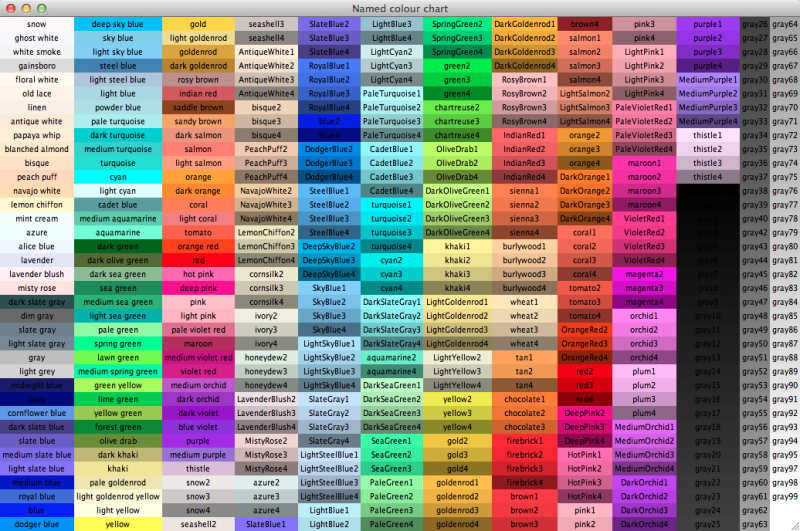
\includegraphics[scale=0.57]{colorchart.png}

\columnbreak

\begin{kod}
  \sor{\pdef~negyzet2(x,~y,~meret):}
  \sor{~~~~t.goto(x,~y)}
  \sor{~~~~t.pendown()}
  \sor{~~~~\pfor~i~\pin~\prange(4):}
  \sor{~~~~~~~~t.forward(meret)}
  \sor{~~~~~~~~t.right(90)}
  \sor{~~~~t.penup()}
  \sor{}
  \sor{\pfor~i~\pin~\prange(20,~320,~20):}
  \sor{~~~~negyzet2(i*-1,~i,~i*2)}
\end{kod}

\end{multicols*}
\end{document}
